
%(BEGIN_QUESTION)
% Copyright 2014, Tony R. Kuphaldt, released under the Creative Commons Attribution License (v 1.0)
% This means you may do almost anything with this work of mine, so long as you give me proper credit

A General Electric model IBC directional overcurrent relay is connected to a current transformer, with the following circuit values.  Note in particular the $R$ and $X_L$ values internal to the CT, representing secondary winding resistance and leakage inductance, respectively:

$$\includegraphics[width=15.5cm]{i00829x01.eps}$$

Calculate the amount of current in the CT secondary circuit, as well as the voltage output by the CT, assuming a perfect 600:5 current ratio for the CT:

\vskip 10pt

$I_{sec} = $ \underbar{\hskip 50pt}

\vskip 10pt

$V_{terminals} = $ \underbar{\hskip 50pt}

\vskip 20pt \vbox{\hrule \hbox{\strut \vrule{} {\bf Suggestions for Socratic discussion} \vrule} \hrule}

\begin{itemize}
\item{} Calculate the C-class required of this CT to avoid undue error under fault conditions, assuming a maximum fault current of 9 kA.
\end{itemize}

\underbar{file i00829}
%(END_QUESTION)





%(BEGIN_ANSWER)

$I_{sec} = $ \underbar{3.56667 A $\angle$ $-116^o$}

\vskip 10pt

$V_{terminals} = $ \underbar{2.275 V $\angle$ $-67.19^o$}

\vskip 10pt

If you attempted to calculate terminal voltage ($V_{terminals}$) by multiplying current and CT winding impedance ([3.56667 A $\angle$ $-116^o$] $\times$ [0.35 $\Omega$ + j0.12 $\Omega$]), you are making a serious mistake.  What this calculation does is calculate the amount of voltage {\it dropped across the winding impedance}, not the voltage seen between the two terminals of the CT.  Bear in mind that the CT winding is the only source in the secondary circuit, everything else in that circuit is a load.

%(END_ANSWER)





%(BEGIN_NOTES)

Secondary current will simply be $5 \over 600$ that of the primary (power line) current, with no phase shift.  Remember that a CT acts as a {\it current source}, and so will ideally output the correct amount of current regardless of burden.

\vskip 10pt

$V_{terminals}$ is simply equal to the circuit current multiplied by the total impedance of wires and relay (total burden) ($V = IZ$):

$$\includegraphics[width=15.5cm]{i00829x02.eps}$$

$$Z_{burden} = (0.22 + j0 \> \Omega) + (0.2 + j0 \> \Omega) + (0 + j0.48 \> \Omega)$$

$$Z_{burden} = 0.42 + j0.48 \> \Omega = 0.6378 \> \Omega \angle 48.81^o$$

\vskip 10pt

$$V_{terminals} = I Z_{burden}$$

$$V_{terminals} = (3.56667 \hbox{ A} \angle -116^o) (0.6378 \> \Omega \angle 48.81^o)$$

$$V_{terminals} = 2.275 \hbox{ V} \angle -67.19^o$$

%INDEX% Electronics review: 3-phase voltage/current/power calculation
%INDEX% Electronics review: AC reactance and impedance
%INDEX% Electronics review, phasor expressions of circuit quantities
%INDEX% Electronics review: series and parallel AC circuits

%(END_NOTES)


